\section{Feigenbaum's Theory of Scaling}

The whole of bifurcation theory is spectacular; even more amazing are the Feigenbaum constants $\alpha$ and $\beta$, whose existence and universality are demonstrated by the numerics in table \ref{tab:feigenbuam_alpha_table_for_logistic} and \ref{tab:feigenbuam_constants_skewed_logistic_map}.
The proof that these constants exist and are universal is well beyond the scope of this undergraduate project, but we can give some rational argument as to the existence of $\alpha$.

\begin{figure}
    \centering
    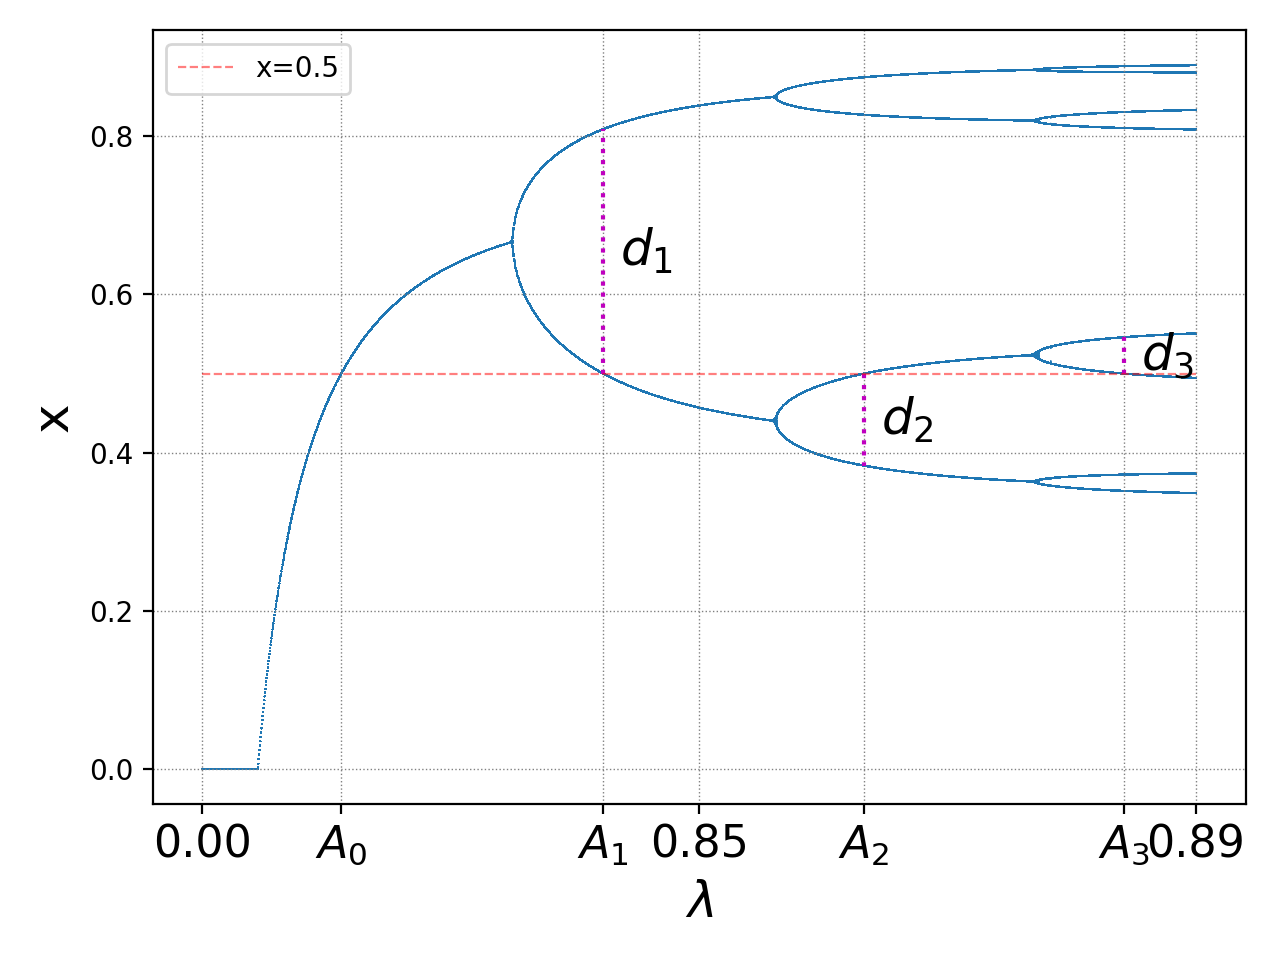
\includegraphics[width=0.6\linewidth]{Images/demonstration of feigenbaum constants.png}
    \caption{Bifurcation diagram of the logistic map which shows the location for $A_n$ and $d_n$ for the first 3 period doubling bifurcations.}
	\label{fig: universal raito}
\end{figure} 

Recall that $\alpha = \lim_{i \rightarrow  \infty}\frac{b_i}{b_{i-1}}$. 
For a given iterative map $F$, depending on one parameter satisfying the requirement of \ref{th:criteria_for_infinite_bifurcations}, $b_i$ is the distance at the superstability of the $2^{i}$ cycle between $X_{m}$ and its closest point in the cycle, where $X_m$ is the unique maximum of $F$.

Writing it in another way
\begin{equation}\label{eq:d_sim}
d_r \sim\frac{D}{(-\alpha)^r} \quad \quad \text{ as } r \to \infty
\end{equation}
where $D$ is a constant depending on $F$ and $\alpha$ is the Feigenbaum's constants. 

Theorem \ref{th:logistic_bifurcation}.\ref{log_closest_branch} states that $d_i = F^{2^{n-1}}(A_i, X_m) - X_m$, where $A_i$ is the value of the parameter at which the $2^n$ cycle achieves superstability and crosses $X_m$ (see figure \ref{fig: universal raito}). 
Therefore, to find the scaling of $d_r$, we take the limit of \eqref{eq:d_sim},

\begin{equation}
\lim_{r \to \infty} (-\alpha)^r \left(F^{2^r}(A_{r+1}, X_m) - X_m\right) = - \frac{D}{\alpha}.
\end{equation}

This leads to the hypothesis that
$$
g_1(x-X_m)=\lim_{r \to \infty} \{g_{1r}(x-X_m)\},
$$
where
$$
g_{1r}(x-X_m) = (-\alpha)^r \{F^{2r}(A_{r+1}, X_m + (x-X_m)/(-\alpha)^r)-X_m\}.
$$
Let $x-X_m$ be the difference from the point of superstability about the bifurcation to $X_m$. 
From the scaling of $d_r$, this implies that $g_1(0)=-\frac{D}{\alpha}$ and by solving for the first couple of iterations of $g_{1r}(x-X_m)$, we can see a limit emerge for $g_1$.
Feigenbaum said that $g_1$ is dependent on the scaling of $x-X_m$ which shows the behaviour of $F$ near to its maximum. 
Since $g_1$ doesn't matter on the map $F$ we can thus say that this behaviour causes $g_1$ to become universal.

Without loss of any generality we can set $X_m=0$.
The main ideas of scaling $x$ can be seen by the operator $T$, which we define to be
\begin{equation} \label{eq: operator T}
T\psi(x)=-\alpha \psi (\psi(-\frac{x}{\alpha})),
\end{equation}
for all continuous functions $\psi$.
Setting $\psi=g_1$, we have
\begin{align}
    Tg_1 &=-\alpha g_1(g_1(-x/\alpha)) \nonumber \\
    &= -\alpha \lim_{r \to \infty} \{(-\alpha)^rF^{2r}(A_{r+1}, (-\alpha)^rF^{2r}(A_{r+1},x/(-\alpha)^{r+1}))\}.  \label{eq:one}
\end{align}
Now, if we set $\phi(y)=(-\alpha)^rF^{2r}(A_{r+1},y/(-\alpha)^r))\}$ such that $$\phi^2=\phi(\phi(y))=(-\alpha)^rF^{2r+1}(A_{r+1},y/(-\alpha)^r))\}$$ and $y=\frac{x}{\alpha}$, we can see that
\begin{align*}
    Tg_1 &= \lim_{r \to \infty} \{(-\alpha)^{r+1}F^{2r+1}(A_{r+1}, x/(-\alpha)^{r+1})\} \\
    &= \lim_{q \to \infty} \{(-\alpha)^qF^{2q}(A_q,x/(-\alpha)^q)\} \\
    &= g_0(x)
\end{align*}
This then implies that $Tg_k(x)=g_{k-1}(x)$ for $k = 2,3,...$ where we have shown that,
\begin{align}
    g_k=\lim_{r \to \infty} \{(-\alpha)^{r}F^{2r}(A_{r+k}, x/(-\alpha)^{r})\}. \label{eq:two}
\end{align} 
As $k \to \infty$ we can show that there could exist a function $g(x)= \lim_{k \to \infty}g_k(x)$ such that we can create the functional equation,
\begin{align}
    Tg=g \label{eq:FunctionalOperator}
\end{align}
such that we can say there exists a `fixed point' $g$ of the nonlinear functional operator $T$. This tells us that when we apply $T$ to $g$, this doesn't change the inherent properties of $g$. 

Using the functional equation \eqref{eq:FunctionalOperator}, the constant $\alpha$ must be determined as part of the solution. The function $g(x)$ satisfies this functional equation, and it possesses a scaling symmetry, such that if $g(x)$ is a solution, then the rescaled function $\mu g(x/\mu)$ is also a solution for any $\mu \neq 0$. This scaling symmetry implies that there is an inherent freedom in the choice of the parameter $\mu$, meaning the solution is not unique until this freedom is constrained. To fix $\mu$ and ensure a unique solution, we adopt a convention by selecting a specific value of $\mu$ such that the function $g(x)$ satisfies a normalisation condition. Once this value of $\mu$ is chosen, the functional equation determines the value of the constant $\alpha$. Although $\alpha$ can be obtained numerically through the solution of the difference equations, its formal derivation comes from solving the functional equation under the chosen normalisation. Thus for the function $g(x)$ that corresponds to the desired map, we can choose a particular $\mu$ such that,
$$
g(0)=1
$$
and by setting $x=0$ in the functional equation and via the original definition of our operator we have it that,
$$
\alpha = -1/g(1)
$$

Feigenbaum was able to numerically verify the method, where he found that
\begin{align}
    g(x)= 1 - 1.52763x^2 + 0.10482x^4- 0.02671x^6 + \dots .\label{eq:feigenbaum}
\end{align}
that corresponds to the desired $\alpha =-1/g(1)=2.5029$.

\begin{exmp} The Logistic Map

    For the logistic map, we have that $F(a,x)=ax(1-x)$ such that the maximum value is attained at $X_m =1/2$. Thus we are able to replace $x-X_m$ with $x-1/2$. Hence our new function is given as $F(a,x)=a(1/4-x^2)-1/2$, ensuring that the maximum value of our new function occurs at $x=0$. Using equations \eqref{eq:one} and \eqref{eq:two} we can now see that,
    \begin{align}
        g_{10}&=F(A_1,x)=A_1(1/4-x^2)-1/2 \nonumber \\
        g_{11}&=(-\alpha)F^2(A_2,x/(-\alpha)) \nonumber \\
        &= \alpha A_2 \left(\left(A_2 \left(x^{2}/\alpha^2 - 1/4\right) + 1/2\right)^{2} - 1/4\right) + \alpha/2
    \end{align}
    Thus, for $g_{1r}(x)$, we can plot our findings as $r \to \infty$ in the $x, y$ plane where $y=g_{1r}(x)$. 
	When we present our first couple of plots, we can see a clear limiting function $g_{k=1}$ appearing as $r$ increases. Thus from \eqref{eq:two} we can see that, as we increase $k$, the sequence of functions converges to some function $g(x)$. 
	We can see the behaviour of our results in the plots in Figure \ref{fig:unscaled}.
	\begin{figure}
    \centering
    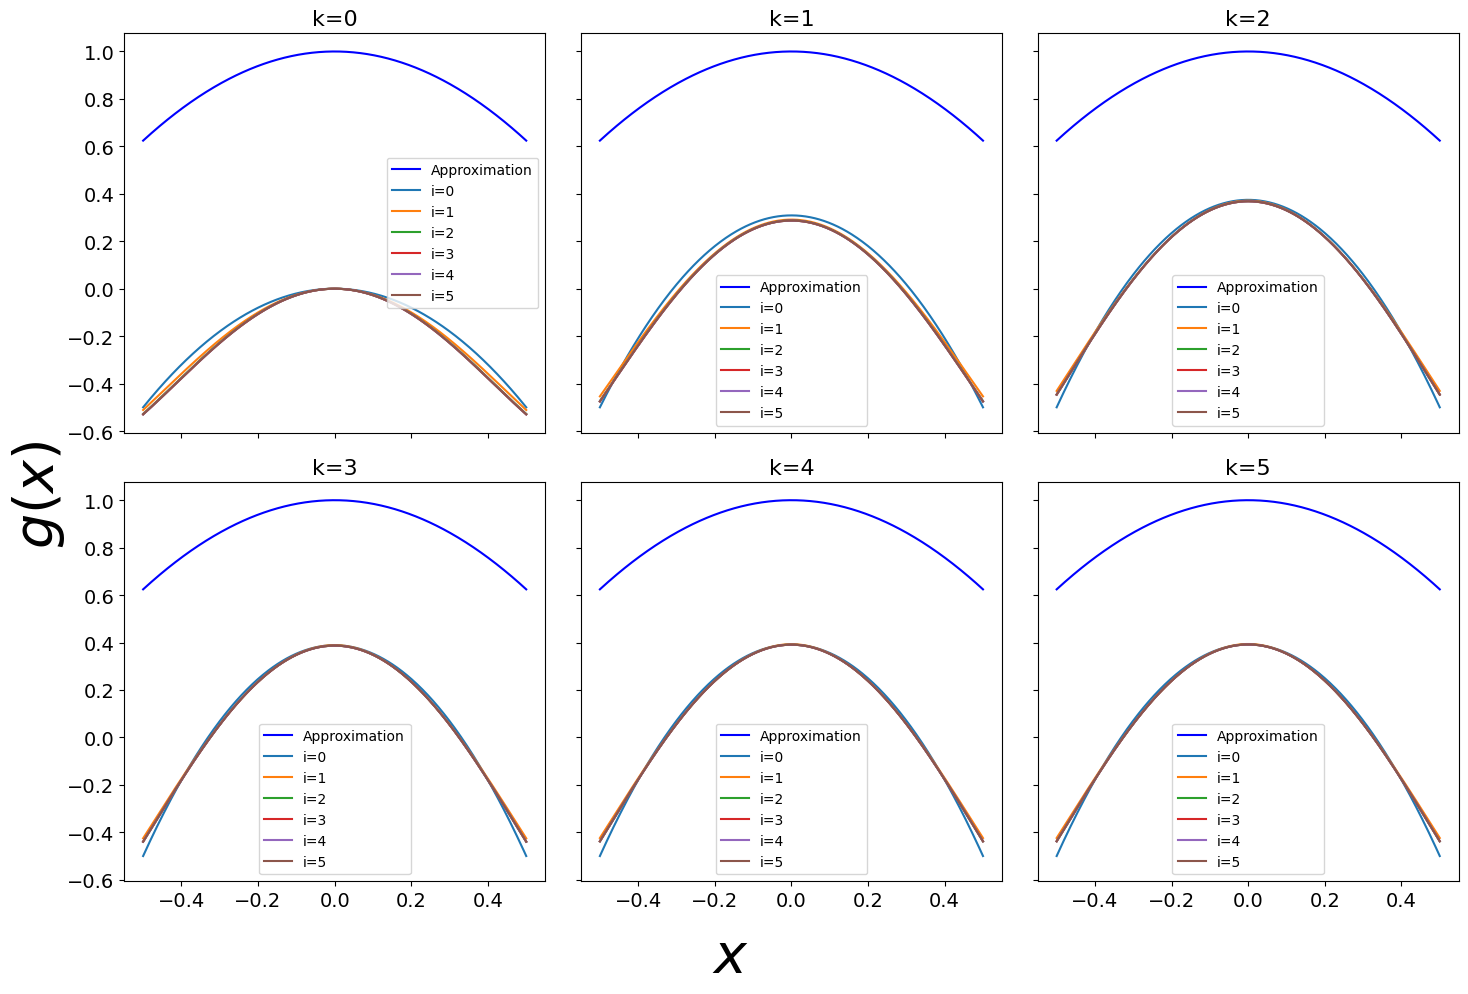
\includegraphics[width=1\textwidth]{Feigenbaum Approx Graphs/Images/feigenbaum.png}
    \caption{Unscaled graphs corresponding to the logistic map}
    \label{fig:unscaled}
\end{figure}
    

    The blue line shows us Feigenbaum's numerically solved solution \eqref{eq:feigenbaum} while the rest of the lines show us the iterations of $r$ for specified $k$ values. 
	We can see that our results produce a correct solution; as we iterate $r$, we can see that our plots converge. However, we can clearly see that our plots don't converge to the desired solution found by Feigenbaum \eqref{eq:feigenbaum}. Since we know, by the universality of the approach, that there exists a scaling factor. From the non linear function operator \eqref{eq:FunctionalOperator}, there exists some scaling factor $\mu$. Thus our solution corresponding to the logistic map has an equivalent solution that matches the one found by Feigenbaum. Since we know $g(0)=1$, we have that $Tg(0)=\mu g(0)$ implies $\mu = 1/g(0)$, where $g(0)$ here is our map's solved unscaled value at 0. From our findings, we found that our value of $g(0)$ is $0.39176186028018406$ such that the corresponding scaling factor was found to be $\mu= 2.552571093277968$. Now that we have our new rescaled function $g(x)$, we can plot the iterations of $r$ and $k$. The results are shown in Figure \ref{fig:rescaled}.
    \begin{figure}
    \centering
    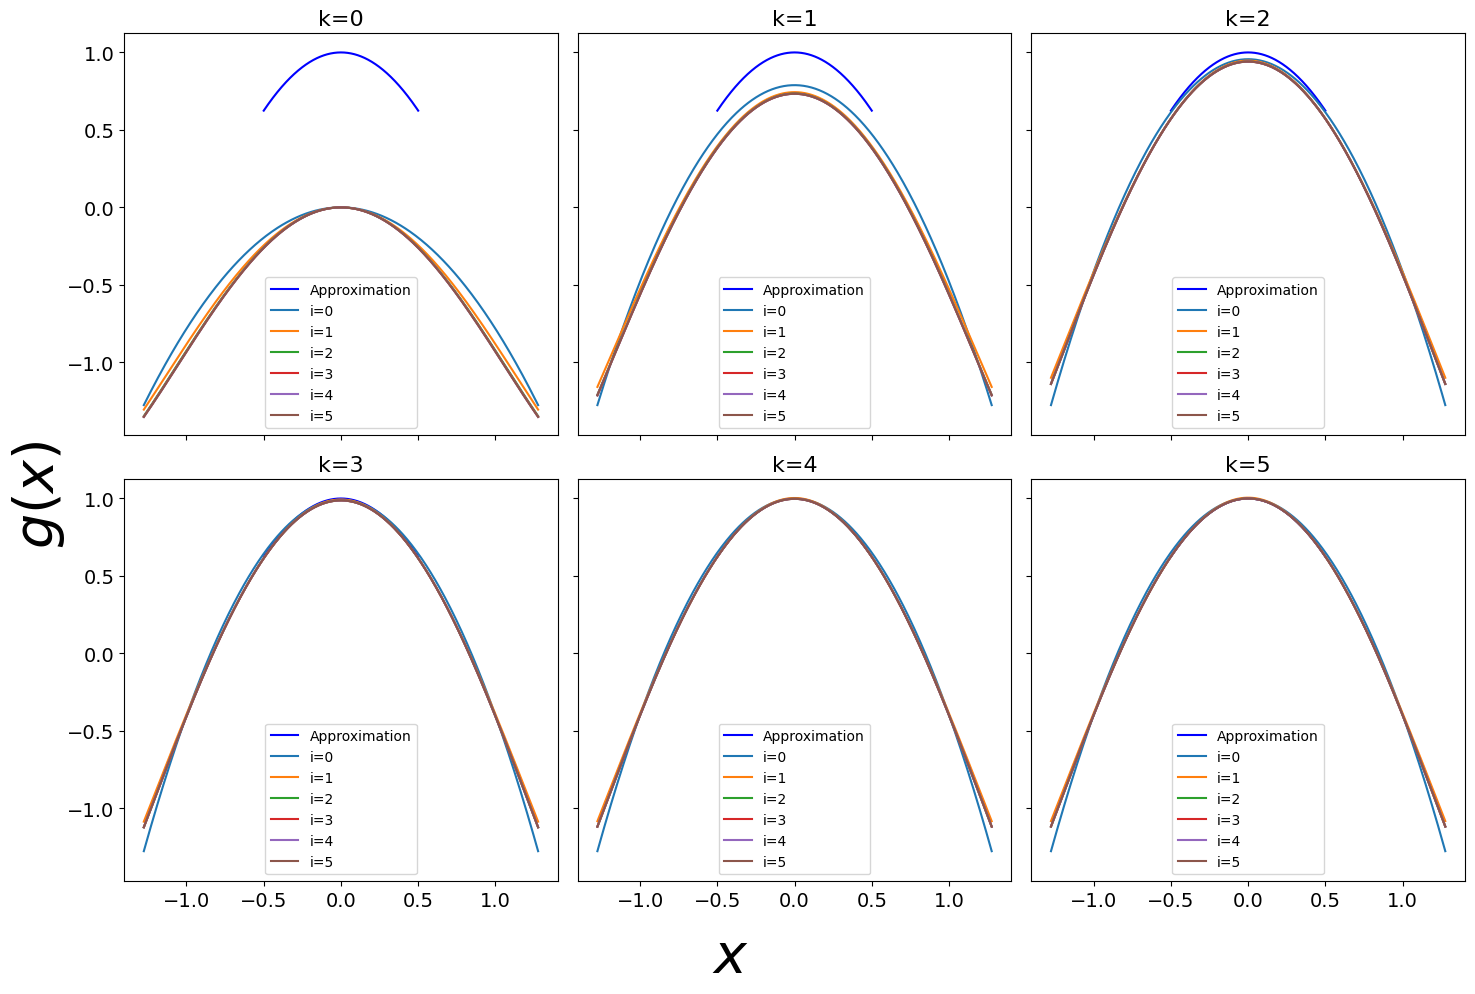
\includegraphics[width=1\textwidth]{Feigenbaum Approx Graphs/Images/fiegenbaum_scaled.png}
    \caption{Rescaled graphs corresponding to the logistic map}
    \label{fig:rescaled}
\end{figure}
The blue lines again show us Feigenbaum's numerically solved solution \eqref{eq:feigenbaum}. We can now see that due to $\mu$, our rescaled $g(x)$ now shifts up towards the true solution and attains the desired shape showing us that we have successfully rescaled our original solution to the universal one presented by Feigenbaum. Thus we have demonstrated the convergence described by Feigenbaum towards his numerical solution as well as the existence of a limiting function $g(x)$ as we increase both $r$ and $k$ simultaneously. 
\end{exmp}


\section{Numerical Computation of Eigenfunction of $T$}

To make the above section rigorous, and prove the existence of an eigenfunction of the operator $T$, is non-trivial and requires a hundred-page proof \cite{lyubich1999feigenbaum}, let alone finding such a function, and is clearly out of the scope of an undergraduate mathematical report like this one. 
In this section, we will attempt to compute the first few terms of the power series of this eigenfunction.

Assuming $g(0) = 1$ and that $g$ is an even function, (the validity of such assumption is justified by the fact that a successful result was found based on it), it can be written in the form of Taylor expansion 
$$
g = 1 + b_1 x^2 + b_2x^4 + \cdots 
$$
Defining the $n$th partial sum of this power series as $g = 1 + b_1x^2 + \cdots + b_{n-1}x^{2n-2}$, and applying $T$ to $g_n$ will produce another $(2n-2)^2$-degree polynomial whose coefficients depend on $b_1, \cdots, b_{n-1}$ and $\alpha$.
Ignoring the terms of degree higher than $2n-2$, and equating the coefficients of the result with that of $g$ of the same degree will give $n$ functions for $n$ variables, whose solution can be solved numerically. 

We will demonstrate an example for $g_1 = 1 + b_1 x^2$. 

Note 
$$
g_1(-\frac{x}{\alpha}) = 1 + b_1 \frac{x^2}{\alpha ^2}
$$

and, by plugging in,

\begin{align*}
-\alpha g_1(g(-\frac{x}{\alpha})) 
&= -\alpha( 1 + b_1(1+b_1 \frac{x^2}{\alpha^2})^2) \\
&= -\alpha(1 + b_1(1 + b_1^2\frac{x^4}{\alpha^4} + x^2 \frac{2b_1}{\alpha^2})) \\
&= -\alpha (1 + b_1)  - \frac{2b_1^2}{\alpha} x^2 - \frac{b_1^3}{\alpha^3}x^4
\end{align*}

thereby comes the equation 

$$
\begin{cases}
    1 &= -\alpha(1+b_1) \\
    b_1 &= -\frac{2b_1^2}{\alpha} 
\end{cases}
$$

The solution is $\alpha = 1 + \sqrt{3} \approx 2.732$ and $b_1 = - \frac{\sqrt{3}}{2} - \frac{1}{2} \approx -1.366$.

Calculating any more terms by hand would be an extremely tedious process, luckily we can resort to computer algebra system for symbolic manipulation (we used Sympy) and BLAS library (fsolve from Scipy) for solving equations of $n$ variables. 
The approximation for the fifteen term is shown in table \ref{tb:b_i table}.
The python code for producing these results is included in Appendix B.

\begin{table}
\centering
\begin{tabular}{|c|c|}
\hline
$n$ & $b_n$ \\
\hline
1 & \( -1.527632997 \times 10^{0} \) \\
2 & \( 1.048151948 \times 10^{-1} \) \\
3 & \( 2.670567058 \times 10^{-2} \) \\
4 & \( -3.527409767 \times 10^{-3} \) \\
5 & \( 8.160111810 \times 10^{-5} \) \\
6 & \( 2.528490972 \times 10^{-5} \) \\
7 & \( -2.556150238 \times 10^{-6} \) \\
8 & \( -9.664817874 \times 10^{-8} \) \\
9 & \( 2.828824961 \times 10^{-8} \) \\
10 & \( -3.352250769 \times 10^{-10} \) \\
11 & \( -2.716117768 \times 10^{-10} \) \\
12 & \( 1.171671302 \times 10^{-11} \) \\
13 & \( 7.447301044 \times 10^{-12} \) \\
14 & \( -2.868216370 \times 10^{-12} \) \\
15 & \( 9.052335129 \times 10^{-13} \) \\
\hline
\end{tabular}
\caption{The values of $b_n$ is the coefficients for the Taylor expression of $g$, where $g$ is the solution to $Tg = g$.
(That is $g = 1 + \sum_{i=1}^n b_i x^{2i}$)}
\label{tb:b_i table}
\end{table}